% !TEX program = xelatex

\documentclass{article}
\usepackage{amsfonts,amssymb}
\usepackage{amsmath}
\usepackage{amsthm}
\usepackage[left=1.0cm,right=1.0cm,top=1.3cm,bottom=1.3cm]{geometry}
\usepackage{enumerate}
\usepackage{fancyhdr}
\usepackage{ctex}
\usepackage{xpatch}
\usepackage{graphicx} %插入图片的宏包
\usepackage{float} %设置图片浮动位置的宏包
\usepackage{subfigure} %插入多图时用子图显示的宏包


\newtheoremstyle{break}
    {\topsep}{\topsep}%
    {\itshape}{}%
    {\bfseries}{}%
    {\newline}{}%
\theoremstyle{break}
\newtheorem*{solution*}{\textbf{Solution:} }
%\newtheorem*{proof*}{\textbf{Proof:}}
\makeatletter

\AtBeginDocument{\xpatchcmd{\@thm}{\thm@headpunct{.}}{\thm@headpunct{}}{}{}}
\makeatother

\pagestyle{fancy}
\lhead{Name}
\chead{\textbf{Discrete Mathematics:  Homework 5}}
\rhead{2020.4.8}
\renewcommand{\baselinestretch}{1.5}

\title{Discrete Mathematics:  Homework 5}
\author{Name  \quad  \quad ID: Number}
\date{2020.4.8}


\begin{document}
\maketitle
\begin{enumerate}
\item Let $p$ be an odd prime and let ${\mathbb{{Z}}_p}^* = \{  [1]_p, [2]_p, \dots , [p-1]_p \}.$
\begin{enumerate}
        \item Show that $([a]_p)^2 = [1]_p$ iff $[a]_p \in \{[1]_p, [p-1]_p\}$.
        \item Show that $[1]_p \cdot [2]_p \cdot \dots [p-1]_p = [-1]_p $ and thus conclude that $(p-1)! \equiv -1 \ (mod \ p) $.
\end{enumerate}
\begin{enumerate}
\item 
\begin{proof}
$[1]_p = 1+np , n \in \mathbb{N}^*.$   $[p-1]_p = p-1+np = (n+1)p -1 .$ $[a]_p = a+np$\\
prove \textbf{IF}:\\
when $a+np=1+np$ , $([a]_p)^2 = (1+np)^2 = 1 + (2n + n^2p)p = [1]+p$\\
when $a+np = (n+1)p -1$ , $([a]_p)^2 = (n^2-1)p+1 = [1]+p$  \\
prive \textbf{ONLY IF}:\\
$[a]_p^2 = a^2 + 2anp + n^2p^2 = a^2 + (2an + n^2p)p = 1 + mp = [1]_p$ where $m,n \in \mathbb{N}^*$\\
so, $a^2 = [1]_p$,$a = [\pm 1]_p$\\
\end{proof}
\item 
\begin{proof}
Because p is an odd prime number, \\
$\mathbb{Z}_p^* = \{1,2, \dots, p-1\}$\\
So $\forall a \in \mathbb{N}^* , 0 < a < p, \exists a^{-1} \in [1,p-1], s.t. \ a a^{-1} \equiv 1 \ (mod \ p)$\\
$\forall a \in (1,p-1)$, we can find a unique $a^{-1} \in (1,p-1)$ \\
By the muplication of $\mathbb{Z}_n$, $[2]_p \cdot \dots [p-2]_p = [1]_p $ \\
And obviously, $[1]_p \cdot [p-1]_p  = [-1]_p$\\
So, $[1]_p \cdot [2]_p \cdot \dots [p-1]_p = [(p-1)!]_p= [-1]_p $  \\
Which equals to $(p-1)! \equiv -1 \ (mod \ p) $\\
\end{proof}
\end{enumerate}
\newpage
\item 
Let $x,y,z$ be integers such that $x^2+y^2 \equiv 3z^2 \ ( mod \ 4)$. Show that $x,y,z$ must be all even.  
Based on this result, show that the equation $x^2+y^2 =3z^2  $ has no other integersolutions
except $(x,y,z) = (0,0,0)$.
\begin{proof}
$x^2+y^2 \equiv 3z^2 \ ( mod \ 4)$, we have$x^2 + y^2 = 3z^2 + 4n, n \in \mathbb{Z}$\\
so, $\frac{x^2+y^2-3z^2}{4}$ is an integer. $4 \mid x^2+y^2-3z^2$\\
if $x,y$ are an odd and an even, $z$ is an even.\\
Suppose $x=2k+1,y=2q,z=2r$, we have $(2k+1)^2 + (2q)^2 - 3(2r)^2 \ mod \ 4 = 1$\\
if $x,y$ are an odd and an even, $z$ is an odd. \\
Suppose $x=2k+1,y=2q,z=2r+1$, we have $(2k+1)^2 + (2q)^2 - 3(2r+1)^2 \ mod \ 4 = 2$\\
if $x,y$ are odds, $z$ is an even.\\
Suppose $x=2k+1,y=2q+1,z=2r$, we have $(2k+1)^2 + (2q)^2 - 3(2r)^2 \ mod \ 4 = 2$\\
if $x,y$ are odds, $z$ is an odd.\\
Suppose $x=2k+1,y=2q+1,z=2r+1$, we have $(2k+1)^2 + (2q)^2 - 3(2r)^2 \ mod \ 4 = 3$\\
where $k,q,r \in \mathbb{Z}$ \\
So, $x,y,z$ must be all even.\\ \\
let $x^2+y^2 \equiv 3z^2 \ ( mod \ 4)$\\
let $x=2k,y=2q,z=2r$, so we have $x^2+y^2 = 4(k^2+q^2) = 12(r^2) = 3z^2$\\ 
and we have $k^2 + q^2 =3r^2$ \\
and $|k|<|x|, |q|<|y|, |r|<|z| $ or $k=x=0, q=y=0, r=z=0$\\
Assume the smallest integer positive solution is $x_0,y_0,z_0$, but there exists $k_0 = \frac 12 x_0, q_0 = \frac 12 y_0, r_0 = \frac 12 z_0$ .\\
So nonzero integer solution doesn't exists.\\
$(x,y,z) = (0,0,0)$ \\
\end{proof}
\newpage
\item 
Let $ a_1,a_2,a_3,a_4 $ be arbitrary integers.  Find ALL integer solutions of the following equation system.
$$
\left\{
\begin{aligned}
        x \equiv a_1 \pmod {11};\\
        x \equiv a_2 \pmod {13};\\
        x \equiv a_3 \pmod {17};\\
        x \equiv a_4 \pmod {19};\\
\end{aligned}
\right.
$$
\begin{solution*}
$n = 11 \cdot 13 \cdot 17 \cdot 19 = 46189$\\
$m_1 = 4199 \quad m_2 = 3553 \quad m_3 = 2717 \quad m_4 =2413$\\
$m_1^{-1}  = 7  \quad m_2^{-1} = 10 \quad m_3^{-1} = 11 \quad m_4^{-1} = 18$ \\
$c_1 = 29392 \quad c_2 = 35530 \quad c_3 = 29887  \quad c_4 =  43758$ \\
$a = \sum_{i=1}^{4} a_i c_i  \pmod n= 29392a_1 + 35530a_2 + 29887a_3 +  43758a_4 \pmod{ 46189}$\\
$x \in [29392a_1 + 35530a_2 + 29887a_3 +  43758a_4 ]_{46189} $
\end{solution*}
\item 
A composite integer $N$ that satisfies the congruence $b^{N−1} \equiv  1 \ (mod \ N$) for all positive 
integers $b$ with $gcd(b,N) = 1 $ is called a Carmichael number.  Suppose that $N=p_1p_2p_3$ is an integer, 
where $p_1$, $p_2$, $p_3$ are primes such that $(p_i−1)|(N−1)$ for $i= 1,2,3$.  Show that $N$ is a Carmichael number. 
\begin{proof}
By Fermat's Little Theorem, we have, \\
$b^{p_1-1}  \equiv 1 \pmod {p_1}$ \\
$b^{p_2-1}  \equiv 1 \pmod {p_2}$ \\
$b^{p_3-1}  \equiv 1 \pmod {p_3}$ \\
$N -1= \mathbb{Z}(p_i-1)$ , $b^{N-1} = b^{\mathbb{Z}(p_i-1)}$\\
$\forall x \equiv 1 \pmod{y}$, we have $x^n \equiv 1 \pmod{y}$ Because $x = 1 + \mathbb{Z}y$ and $x^n = 1 + (2y + \mathbb{Z} y^2)\mathbb{Z}$\\
$\forall x \equiv 1 \pmod y $, we have $x \equiv  1 \pmod{ ky}$ Because $x = 1 + \mathbb{Z}y$ and $x = 1 + \mathbb{Z}y +  \mathbb{Z}y$ \\
So, $b^{N-1} \equiv b^{3(N-1)} \equiv b^{p_1-1}b^{p_2-1}b^{p_3-1} \pmod{p_1p_2p_3}  $\\
Which has the same reminder $1$ as $b^{p_1-1}  \equiv 1 \pmod {p_1}$ \\
So, $b^{N−1} \equiv  1 \ (mod \ N$) \\
So, $N$ is a Carmichael number. 
\end{proof}
\newpage
\item 
See the following figure.  The RSA public keys of Alice, Bob and Charlie are $pk1=(N_1,3)$,
$pk2= (N_2,3)$ and $pk3= (N_3,3)$, respectively.  David wants to send a private message $m$ to Alice, 
Bob and Charlie, where $m$ is an integer and $0< m < N_i$ for $i= 1,2,3$.  In order to keep $m$ secret from
 an eavesdropper Eve, David encrypts $m$ as $ c_1=m^3 \bmod N_1$, $c_2=m^3 \bmod N_2$ and $c_3=m^3 \bmod N_3$; 
 and then sends $c_1$to Alice, $c_2$ to Bob and $c_3$ to Charlie. 

 {\centering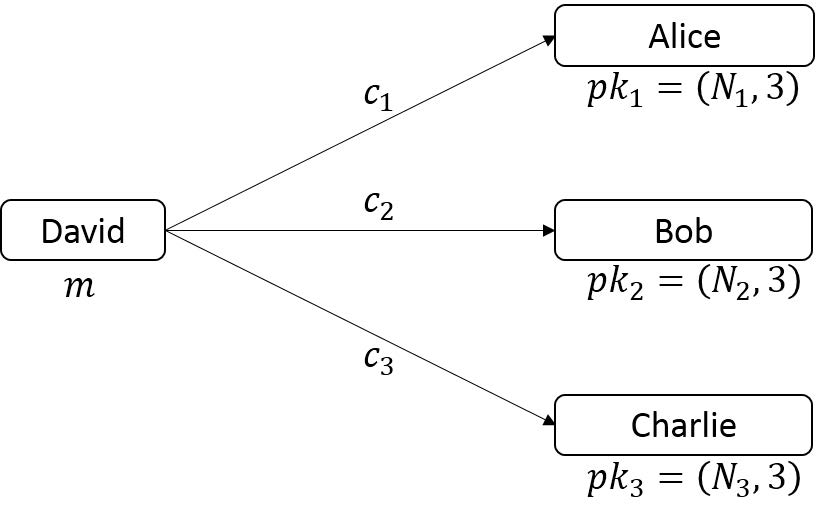
\includegraphics[scale=1]{5.jpg}
 
 }
 Suppose  that $N_1,N_2,N_3$ are  pairwise  relatively  prime.   Show  that  with
the  knowledge  of  all public keys and all ciphertexts, Eve can decide the value of $m$.
\begin{proof}
    By RSA Theorem, we have\\
    $$
    \left\{
    \begin{aligned}
        x^3 \equiv c_1 \pmod {N_1 }\\
        x^3 \equiv c_2 \pmod {N_2 }\\
        x^3 \equiv c_3 \pmod {N_3} \\
    \end{aligned}
    \right.
    $$
    so, 
    $n = N_1N_2N_3$\\
    $m_1 = N_2N_3 \quad m_2 = N_1N_3\quad m_3 = N_1N_2$\\
    % $m_1^{-1}  = 7  \quad m_2^{-1} = 10 \quad m_3^{-1} = 11 \quad m_4^{-1} = 18$ \\
    $c_1 = m_1 m_1^{-1} \quad c_2 = m_2 m_2^{-1}  \quad c_3 = m_3  m_3^{-1} $ \\
    $a = \sum_{i=1}^{k} a_i c_i  \pmod n$\\
    $x^3 \in [ \sum_{i=1}^{3} a_i c_i  ]_{n} $\\
    so we can try to solve every x as a message. \\
\end{proof}
\newpage
\item 
See the following figure.  Alice and Bob trust each other very much.  
They set their RSA  public  keys  as $pk1=  (N,e1) $ and  $pk2=  (N,e2)$,  respectively. 
  Charlie  wants  to  send  aprivate message $m$ to Alice and Bob,
   where $0 \leq m < N$ is an integer and $gcd(m,N) = 1$.  
   In order to keep $m$ secret from an eavesdropper Eve,
    Charlie encrypts $m $ as $c_1=m^{e1} \bmod N$ and 
    $c_2=m^{e2} \bmod N$; and then sends $c1$ to Alice and $c2$ to Bob.

    {\centering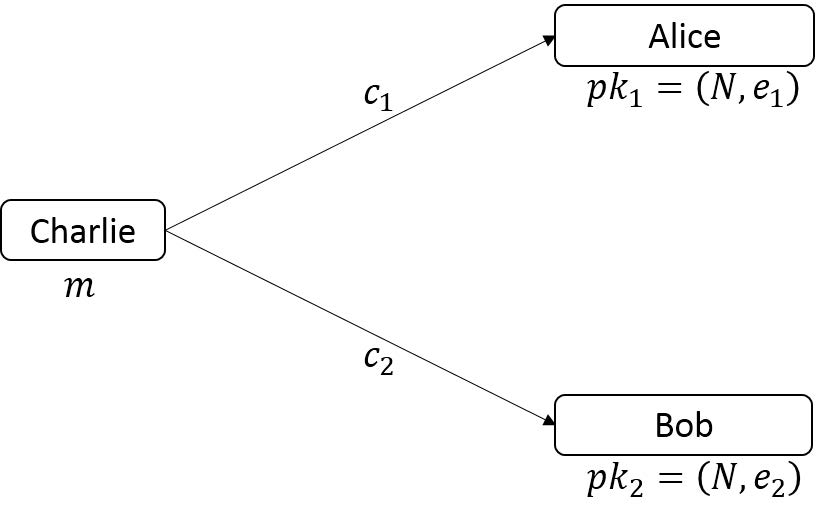
\includegraphics[scale=1]{6.jpg}
 
    }
    Suppose that $gcd(e1,e2) = 1$. Show that with the knowledge of all public keys 
    and all ciphertexts, Eve can decide the value of $m$.
    \begin{proof}
        By RSA Theorem, we have\\
        $$
        \left\{
        \begin{aligned}
            x^{e_1} \equiv c_1 \pmod {N}\\
            x^{e_2} \equiv c_2 \pmod {N }\\
        \end{aligned}
        \right.
        $$
    \end{proof}
    Because $gcd(e_1, e_2) =1$, we have $x_1e_1+y_1e_2 = gcd(e_1, e_2) =1$ by EXGCD.\\
    so, $x^{x_1e_1+y_1e_2} \equiv c_1^{x_1} + c_2^{x_2} \equiv x^{1} \equiv \pmod{N}$ , and $N$ is a prime.
    so, Eve can solve $m$ by solving $m \equiv c_1^{x_1} + c_2^{x_2}  \pmod{ N} $\\
\end{enumerate}
\end{document}